\documentclass[conference,10pt]{IEEEtran}
\IEEEoverridecommandlockouts

\usepackage[T1]{fontenc}
\usepackage{amsmath,amssymb,amsthm}
\usepackage{graphicx}
\usepackage{booktabs}
\usepackage{multirow}
\usepackage{array}
\usepackage{algorithm}
\usepackage{algpseudocode}
\usepackage{tikz}
\usetikzlibrary{arrows.meta,positioning,fit,calc,shapes.geometric}
\usepackage[hidelinks]{hyperref}
\usepackage{cite}
\usepackage{xcolor}

\newtheorem{definition}{Definition}
\newtheorem{lemma}{Lemma}
\newtheorem{proposition}{Proposition}
\newtheorem{theorem}{Theorem}
\newtheorem{corollary}{Corollary}
\theoremstyle{remark}
\newtheorem{remark}{Remark}

\newcommand{\Qs}{Q_{\mathrm{step}}}
\newcommand{\SSE}{\mathrm{SSE}}
\newcommand{\PSNR}{\mathrm{PSNR}}
\newcommand{\HMAC}{\mathsf{HMAC}}
\newcommand{\Hash}{\mathsf{SHA256}}
\newcommand{\Pos}{\mathsf{Poseidon}}
\newcommand{\dig}{\mathsf{dig}}
\newcommand{\bind}{\mathsf{bind}}
\newcommand{\cat}{\,\|\,}

\begin{document}

\title{Covert, Anonymous and Video-Bound Provenance:\\
Hiding zk-SNARK Camera Proofs in H.264 CAVLC Trailing-One Signs}

\author{\IEEEauthorblockN{Author Name(s) (to be filled in)}
\IEEEauthorblockA{Affiliation\\
City, Country\\
e-mail}}

\maketitle

\begin{abstract}
Deployed content-provenance systems attach a signed manifest to a media file. The manifest is metadata that platforms strip, it identifies the signing device, and its presence is visible. We hide a zero-knowledge proof of origin inside the H.264 bitstream instead. A camera whose key is a leaf of a public Poseidon Merkle registry produces a 129-byte Groth16 proof that it is registered and vouches for a binding of the video and a message; the proof is embedded, under a separate stego key, into CAVLC trailing-one signs of IDR frames, which keeps every codeword length and the file size. To bind the proof to the stream that carries it, we hash every NAL unit with exactly the keyed carrier bits cleared: the digest is invariant under embedding, while any other edit---another video, truncation, re-encoding, an edited non-carrier bit---changes it. Verifiers need the stego key and the registry root but no camera secret, cannot forge proofs and do not learn which camera signed. We also derive a closed-form distortion model: one sign flip costs $4\Qs^2\kappa$ in pixel energy, $\kappa\in[0.925,1.057]$, times a propagation gain $G$, which inverts into a per-frame bit budget for a target PSNR. On 1{,}200 single flips and 810 frames the direct energy matches the decoder exactly, $G$ does not depend on QP, and its heavy-tailed distribution---a tenth of the carriers causes four fifths of the distortion---predicts frame distortion. A 68-byte message and its proof occupy 26 IDRs with a minimum PSNR-Y of 44.03\,dB; proving takes 1.5--1.8\,s, verification about 1\,s, and an 11-case attack matrix including replay is rejected as expected.
\end{abstract}

\begin{IEEEkeywords}
Video steganography, H.264/AVC, CAVLC, zk-SNARK, Groth16, content provenance, anonymous attestation, distortion model.
\end{IEEEkeywords}

\section{Introduction}
\label{sec:intro}

Whether a video was really captured by a trustworthy device has become a practical question for newsrooms, courts and platforms. The industry answer is the C2PA standard~\cite{c2pa_spec}: the capture device signs a manifest that binds a hash of the asset to assertions about its origin, and the manifest travels with the file as metadata. This design has three properties that are undesirable in some settings. First, the manifest is \emph{separable}: social networks and many transcoding pipelines strip metadata, which is why C2PA added watermark-based ``soft bindings'' to recover a lost manifest. Second, it is \emph{identifying}: the signature is verified against a device or vendor certificate, so the verifier learns who signed. Third, it is \emph{visible}: anyone can see that the file carries provenance, and an adversary who wants to suppress it knows exactly which files to target.

Zero-knowledge proofs address the second point. A camera can prove that it belongs to a set of authorized devices without revealing which one, the pattern behind anonymous credentials and Semaphore-style group membership~\cite{zerocash2014,semaphore}. Recent work applies zk-SNARKs to media provenance, mostly to prove that a published image or video is a permissible transformation of a signed original~\cite{photoproof2016,zkimg2022,veritas2024,vimz2024,zkcinema2026,aipa2026}. Steganography addresses the first and third points: a message hidden in the coded bitstream survives metadata stripping and container changes, and is invisible to a party that does not hold the key~\cite{simmons1984,cachin1998,fridrich2009book}. Compressed-domain data hiding in H.264 has a long history, including embedding in the sign bits of CAVLC trailing ones, which leaves the bit rate unchanged~\cite{kapotas2007,mobasseri2007,fragile_h264_mtap}.

This paper combines the two. The question we answer is: \emph{can a short zero-knowledge proof of anonymous camera membership be hidden inside the H.264 bitstream it vouches for, bound to that exact bitstream, at a quality cost that can be predicted and controlled?} Three technical obstacles stand in the way. (i)~A proof embedded into a video changes the video, so a proof that commits to the video's hash cannot be computed before embedding; the binding has to be defined over a canonical form that embedding leaves unchanged, without opening a gap an attacker can exploit. (ii)~The proof must be small enough for a covert channel whose capacity is a few dozen bits per frame, and its verifier must not need the camera's secret---otherwise any verifier could forge proofs, and the proof would add nothing over a shared-key MAC. (iii)~Sign flips in intra-coded frames propagate through intra prediction, so the quality cost is not simply proportional to the number of embedded bits; it must be modeled before an embedding budget can be chosen.

\textbf{Contributions.}
\begin{itemize}
\item A \emph{video-bound anonymous camera proof} (Section~\ref{sec:design}): a Circom circuit of 8{,}737 constraints with three public inputs (registry root and a 256-bit binding split in two halves) proving that $\Pos(s)$ is a leaf of a depth-16 Poseidon Merkle registry, with Groth16 proofs of 129 bytes.
\item A \emph{carrier-masked video digest}: SHA-256 over the RBSP of every NAL unit with exactly the keyed carrier bits cleared. We prove that it is invariant under embedding and that every other edit is detected, either through the digest or through the extracted proof input (Section~\ref{sec:security}).
\item A \emph{keyed, segment-wise covert channel} on CAVLC trailing-one signs with HKDF-derived schedule and whitening keys, a three-byte frame, and one segment per IDR, which works identically on files and on live streams.
\item A \emph{closed-form distortion model} of trailing-one sign embedding, derived from the H.264 dequantization and inverse transform, together with its inverse: the number of flips, and hence the per-IDR bit cap, that keeps a frame above a target PSNR (Section~\ref{sec:distortion}).
\item An implementation and an evaluation (Sections~\ref{sec:impl}--\ref{sec:eval}): 27 encodes at three resolutions, a model validation on sequence-level and single-flip experiments under two encoder configurations, Groth16/PLONK costs, and an 11-case attack matrix.
\end{itemize}

\textbf{Scope.} The scheme is \emph{fragile} by design: it protects bitstreams that are transferred unchanged (evidence chains, archives, files sent as files). A re-encode destroys both the payload and the digest; robustness to transformations is the subject of the transformation-proof literature~\cite{photoproof2016,veritas2024,zkcinema2026} and is outside this paper. The proof states that a registered camera vouched for a bitstream, not that the scene is real.

\section{Related Work}
\label{sec:related}

\textbf{Data hiding in the H.264 compressed domain.} Embedding directly in entropy-coded syntax avoids a full decode--encode cycle. Kim \emph{et al.}~\cite{kim2007t1} write a bit into the sign of the highest-frequency trailing one of luma blocks, which keeps every codeword length and therefore the bit rate; Lin \emph{et al.}~\cite{lin2012cavlc} embed the XOR of all trailing-one signs of keyed blocks; Wang and Ma~\cite{wang2018cavlc} use one host block out of every $E$ candidates and a $(1,3,2)$ matrix code when a block has three trailing ones; Liao \emph{et al.}~\cite{liao2009t1,liao2012t1journal} hide one bit per intra macroblock in a trailing-one parity. Other CAVLC methods substitute codewords~\cite{mobasseri2007} or modify levels~\cite{fragile_h264_mtap}. Because intra prediction reuses reconstructed neighbors, such changes \emph{drift} inside the frame; Ma \emph{et al.}~\cite{ma2010drift} choose blocks and modify coefficient pairs so that the error cannot propagate (their conditions are tabulated in~\cite{nguyen2022drift}). You \emph{et al.}~\cite{you2017cavlc} show that CAVLC hiding is detectable and propose a detection strategy. We use the trailing-one sign carrier, add a keyed schedule and whitening, quantify drift with an explicit model, and compare against the sign-reducible methods above under identical conditions (Section~\ref{sec:eval}).

\textbf{Fragile watermarking and self-authentication.} A classic construction hashes the content without the embedding region, signs the hash and embeds the signature into that region~\cite{yeung1997,wong1998}. Our video digest follows this pattern, with two differences that matter for security: the excluded region is \emph{only} the set of keyed carrier positions (not a whole bit plane or block class), and the embedded object is a zero-knowledge proof rather than a signature, so verification reveals neither the signer nor a verification key per device.

\textbf{Media provenance.} C2PA~\cite{c2pa_spec} binds signed manifests to assets through hard bindings (hashes) and soft bindings (watermarks or fingerprints). It offers public verifiability and an established certificate infrastructure, but the manifest is separable metadata and the signer is identified. Our proof travels inside the bitstream, is hidden from parties without the stego key, and hides the signer within the registry.

\textbf{Zero-knowledge proofs for media.} PhotoProof~\cite{photoproof2016} proves that an image is derived from a signed original by permissible transformations. ZK-IMG~\cite{zkimg2022} attests images from attested cameras and hides the pre-image of transformations; VerITAS~\cite{veritas2024} and VIMz~\cite{vimz2024} scale such proofs to high-resolution images, the latter with folding-based SNARKs and signer anonymity; zk-Cinema~\cite{zkcinema2026} extends transformation proofs to video; AIPA~\cite{aipa2026} adds unlinkable pseudonym certificates. These systems prove \emph{what happened to} a signed asset and keep the proof beside it. We solve a different problem: the proof is hidden \emph{inside} the asset, bound to the exact bitstream, and the signer is anonymous within a registry; we do not support transformations.

\textbf{Zero knowledge and information hiding.} Adelsbach and Sadeghi~\cite{adelsbach2001zkwm} prove the presence of a watermark in zero knowledge; Toso and Chung~\cite{toso2006} combine steganography and an interactive zero-knowledge proof to embed a signature in an image. We embed a non-interactive succinct argument whose statement depends on the cover itself.

\textbf{Anonymous membership.} Proving that a committed key is a leaf of a public Merkle tree~\cite{merkle1987} without revealing the leaf is the core of Zerocash~\cite{zerocash2014} and Semaphore~\cite{semaphore}; Poseidon~\cite{poseidon2021} makes the in-circuit hashing cheap. We use this pattern for a camera registry.

\textbf{Minimal-distortion steganography.} Matrix embedding~\cite{westfeld2001f5} and syndrome-trellis codes~\cite{filler2011stc,fridrich2007practical} minimize an additive distortion for a given payload. Our model supplies the per-carrier cost such codes need in the CAVLC sign domain.

Table~\ref{tab:related} summarizes the comparison.

\begin{table*}[t]
\centering
\caption{Comparison with provenance and compressed-domain hiding approaches. \checkmark: supported; --: not supported; (\checkmark): partially.}
\label{tab:related}
\small\setlength{\tabcolsep}{4pt}
\begin{tabular}{@{}p{4.6cm}*{6}{>{\centering\arraybackslash}p{1.65cm}}@{}}
\toprule
Approach & In-band (no metadata) & Hidden & Signer anonymous & Bound to exact stream & Survives re-encode & Public verification \\
\midrule
C2PA manifest~\cite{c2pa_spec} & -- & -- & -- & \checkmark & (\checkmark)$^a$ & \checkmark \\
CAVLC fragile watermark~\cite{mobasseri2007,fragile_h264_mtap} & \checkmark & (\checkmark) & -- & \checkmark & -- & -- \\
CAVLC sign/parity hiding~\cite{kim2007t1,lin2012cavlc,wang2018cavlc,liao2012t1journal} & \checkmark & \checkmark & -- & -- & -- & -- \\
Signed digest in content~\cite{wong1998} & \checkmark & -- & -- & \checkmark & -- & \checkmark \\
PhotoProof / ZK-IMG~\cite{photoproof2016,zkimg2022} & -- & -- & (\checkmark) & -- & \checkmark$^b$ & \checkmark \\
VIMz / zk-Cinema / AIPA~\cite{vimz2024,zkcinema2026,aipa2026} & -- & -- & \checkmark & -- & \checkmark$^b$ & \checkmark \\
\textbf{This work} & \checkmark & \checkmark & \checkmark & \checkmark & -- & (\checkmark)$^c$ \\
\bottomrule
\end{tabular}

\vspace{2pt}{\footnotesize $^a$ via soft-binding watermarks that recover the manifest. $^b$ for the transformations the proof system supports. $^c$ per video, through a disclosed verification token (Section~\ref{sec:params}); otherwise verifiers need the stego key.}
\end{table*}

\section{Background}
\label{sec:background}

We summarize the parts of H.264/AVC~\cite{itu_h264,wiegand2003overview,richardson2010h264} that the channel and the distortion model rely on, and the zero-knowledge tools of the proof. We restrict attention to the Constrained Baseline profile: progressive 4:2:0, 8-bit, CAVLC entropy coding, flat scaling matrices.

\subsection{Intra coding of an IDR picture}
An IDR picture is split into $16\times16$ macroblocks (MBs) coded in raster order. In an I-slice an MB is either \emph{Intra4$\times$4} (sixteen $4\times4$ luma blocks, each predicted with one of nine directional modes from reconstructed samples above and to the left), \emph{Intra16$\times$16} (one of four modes for the whole MB: vertical, horizontal, DC, plane), or I\_PCM. Chroma ($8\times8$ per MB for 4:2:0) uses one of four modes. The encoder codes the prediction residual $e=x-p$; the decoder reconstructs $\hat x=\mathrm{clip}(p+\hat e)$. Because $p$ is computed from \emph{reconstructed} neighbors, a change in $\hat e$ of one block alters the prediction of later blocks: this is intra drift.

\subsection{From the DCT to the integer transform}
The $4\times4$ two-dimensional DCT-II is $Y=AXA^{\top}$ with
\begin{equation}
A=\begin{bmatrix}a&a&a&a\\ b&c&-c&-b\\ a&-a&-a&a\\ c&-b&b&-c\end{bmatrix},\quad
\begin{aligned}a&=\tfrac12,\\ b&=\tfrac{1}{\sqrt2}\cos\tfrac{\pi}{8},\\ c&=\tfrac{1}{\sqrt2}\cos\tfrac{3\pi}{8}.\end{aligned}
\end{equation}
H.264 replaces $c/b\approx0.414$ by $1/2$ and rescales $b=\sqrt{2/5}$ to keep the rows orthogonal~\cite{malvar2003transform}. The transform factors into an integer core and a scaling that is folded into quantization:
\begin{equation}
Y=\left(C_f\,X\,C_f^{\top}\right)\odot E_f,\qquad
C_f=\begin{bmatrix}1&1&1&1\\2&1&-1&-2\\1&-1&-1&1\\1&-2&2&-1\end{bmatrix},
\end{equation}
where $E_f$ has entries $a^2$, $ab/2$, $b^2/4$ according to the parity class of $(i,j)$: both indices even, both odd, or mixed. The inverse is
\begin{equation}
X=C_i^{\top}\left(Y\odot E_i\right)C_i,\qquad
C_i=\begin{bmatrix}1&1&1&1\\1&\tfrac12&-\tfrac12&-1\\1&-1&-1&1\\\tfrac12&-1&1&-\tfrac12\end{bmatrix},
\label{eq:inverse}
\end{equation}
with $E_i$ entries $a^2$, $ab$, $b^2$. Only additions and shifts are needed, and encoder and decoder match exactly. We write $b_0,\dots,b_3$ for the rows of $C_i$; their squared norms are $\|b_0\|^2=\|b_2\|^2=4$ and $\|b_1\|^2=\|b_3\|^2=5/2$.

\subsection{Quantization and scaling}
The quantizer step $\Qs$ doubles every six QP values:
\begin{equation}
\Qs(\mathit{QP})=\Qs(\mathit{QP}\bmod6)\cdot2^{\lfloor \mathit{QP}/6\rfloor},
\label{eq:qstep}
\end{equation}
with $\Qs(0..5)=0.625, 0.6875, 0.8125, 0.875, 1, 1.125$. The encoder computes $W=C_fXC_f^{\top}$ and quantizes
\begin{equation}
|Z_{ij}|=\left(|W_{ij}|\,MF_{ij}+f\right)\gg q_{\mathrm{bits}},\quad q_{\mathrm{bits}}=15+\lfloor \mathit{QP}/6\rfloor,
\label{eq:quant}
\end{equation}
with $MF=2^{q_{\mathrm{bits}}}\,PF/\Qs$, $PF\in\{a^2,ab/2,b^2/4\}$, and a dead-zone offset $f$ ($2^{q_{\mathrm{bits}}}/3$ for intra in the reference design; x264 additionally applies trellis and psychovisual decisions). The decoder scales a level $c_{ij}$ by
\begin{equation}
d_{ij}=c_{ij}\cdot v_{m}(i,j)\cdot2^{\lfloor \mathit{QP}/6\rfloor},\qquad m=\mathit{QP}\bmod6,
\label{eq:dequant}
\end{equation}
where $v_m(i,j)\in\{v_{m,0},v_{m,1},v_{m,2}\}$ by parity class (even/even, odd/odd, mixed):
\begin{equation}
\begin{array}{c|cccccc}
m & 0 & 1 & 2 & 3 & 4 & 5\\\hline
v_{m,0} & 10 & 11 & 13 & 14 & 16 & 18\\
v_{m,1} & 16 & 18 & 20 & 23 & 25 & 29\\
v_{m,2} & 13 & 14 & 16 & 18 & 20 & 23
\end{array}
\label{eq:vtable}
\end{equation}
(The standard writes $\mathrm{LevelScale}=16\,v_m$ and a shift by four for flat matrices; the product is the same.) The residual is then $\hat e=(C_i^{\top}D\,C_i+32)\gg6$, where $C_i$ is applied with integer shifts. Note that $\Qs(m)=v_{m,0}/16$: the step size is the even/even scaling factor.

\textbf{DC paths.} In an Intra16$\times$16 MB the sixteen luma DC coefficients form a $4\times4$ block coded separately (category \emph{LumaDC}), transformed by a $4\times4$ Hadamard matrix before scaling; the remaining fifteen coefficients of each block are \emph{Luma AC}. For chroma, the four DC coefficients of each $8\times8$ component form a $2\times2$ block (\emph{ChromaDC}) with a $2\times2$ Hadamard transform, and each $4\times4$ block has fifteen \emph{ChromaAC} coefficients. Chroma uses $\mathit{QP}_c$, derived from $\mathit{QP}+\texttt{chroma\_qp\_index\_offset}$ by a table that saturates at 39.

\subsection{CAVLC}
After a zig-zag scan, each block of levels is coded as~\cite{itu_h264,richardson2010h264}:
\begin{enumerate}
\item \texttt{coeff\_token}: the pair (TotalCoeff, TrailingOnes), from one of four VLC tables chosen by $n_C$, the rounded mean of TotalCoeff of the left and upper blocks;
\item one \texttt{trailing\_ones\_sign\_flag} per trailing one---the up to three highest-frequency non-zero coefficients equal to $\pm1$---in reverse scan order, $0\mapsto+1$, $1\mapsto-1$;
\item the remaining levels (\texttt{level\_prefix}, \texttt{level\_suffix}, adaptive \texttt{suffixLength}), \texttt{total\_zeros} and \texttt{run\_before}.
\end{enumerate}

\begin{proposition}[Syntax invariance]
\label{prop:syntax}
Flipping a \texttt{trailing\_ones\_sign\_flag} changes exactly one level from $\pm1$ to $\mp1$ and leaves the length and the decoded value of every other syntax element of the slice unchanged.
\end{proposition}
\begin{proof}
The flag is a fixed one-bit field. TotalCoeff and TrailingOnes, hence the \texttt{coeff\_token} codeword and the $n_C$ context of later blocks, do not depend on signs. The initial \texttt{suffixLength} depends only on TotalCoeff and TrailingOnes, its updates only on the non-trailing-one levels, and the magnitude adjustment of the first non-trailing-one level only on TrailingOnes. \texttt{total\_zeros} and \texttt{run\_before} depend on positions only. Hence every later bit is parsed at the same offset with the same meaning.
\end{proof}

Consequently the edited stream is a valid stream of the same RBSP length, and the set of trailing-one sign positions (the \emph{candidates}) is the same in the cover and the stego stream. We use the \emph{first} sign flag of each block that has at least one trailing one, i.e.\ the highest-frequency trailing one.

\subsection{NAL units and emulation prevention}
An Annex-B stream is a sequence of NAL units separated by start codes \texttt{00\,00\,01}. Each NAL unit has a one-byte header (\texttt{forbidden\_zero\_bit}, \texttt{nal\_ref\_idc}, \texttt{nal\_unit\_type}) followed by the EBSP: the RBSP with an emulation-prevention byte \texttt{03} inserted after every \texttt{00\,00} that precedes a byte $\le\texttt{03}$. Bit offsets in this paper are RBSP offsets. A sign flip can add or remove one emulation-prevention byte, which changes the file size by one byte but no RBSP offset.

\subsection{zk-SNARKs, Groth16 and Poseidon}
A statement ``$\exists w: \mathcal R(x,w)$'' is compiled to a rank-1 constraint system $(Az)\circ(Bz)=Cz$ over the BN254 scalar field~\cite{bn2005}, $z=(1,x,w)$. Groth16~\cite{groth2016} proves satisfiability with $\pi=(A,B,C)\in\mathbb G_1\times\mathbb G_2\times\mathbb G_1$, verified with one pairing-product equation; it is complete, knowledge-sound and perfectly zero-knowledge in the generic group model. The common reference string comes from a universal Phase~1 (Powers of Tau) and a circuit-specific Phase~2; the multi-party ceremony is secure if one participant is honest~\cite{bowe2017mpc}. A proof compresses to 129 bytes: the $x$-coordinates of $A$, $B$ (two $\mathbb F_q$ elements) and $C$, plus one byte of sign flags. PLONK~\cite{plonk2019} trades a larger proof for a universal setup. Poseidon~\cite{poseidon2021} is a sponge hash over the scalar field designed for few constraints; we use it for public keys and Merkle nodes. Circuits are written in Circom~\cite{circom2023} and proven with snarkjs~\cite{snarkjs}.

\section{System and Threat Model}
\label{sec:threat}

\textbf{Parties.} A \emph{registry authority} publishes the root $\rho$ of a Merkle tree of camera public keys. A \emph{camera} holds a secret $s$ with $\Pos(s)$ in the tree. A \emph{sender} (the camera or an embedder it trusts) holds a 32-byte stego key $K$ shared with the intended verifiers, and turns a cover H.264 stream into a stego stream carrying a message $m$ and a proof. The \emph{channel} delivers the bitstream, possibly through a party that inspects or edits it. A \emph{verifier} knows $K$, $\rho$ and the Groth16 verification key, and accepts or rejects.

\textbf{Two secrets, two roles.} $K$ hides and locates the payload; $s$ authorizes it. Holding $K$ lets a verifier extract and check a proof but not create one, which is the point of using a zero-knowledge proof instead of a MAC under $K$.

\textbf{Adversary.} The adversary sees stego streams and may know $K$ (a curious or malicious verifier) or not (a channel observer). It may edit, truncate, splice or re-encode streams, move a valid payload into another stream, change the message, register its own cameras in a tree of its choice, and obtain proofs from honest cameras for streams of its choice. It does not know the secret of any honest registered camera and cannot break SHA-256, Poseidon, HMAC-SHA256 or the Groth16 assumptions.

\textbf{Goals.}
\begin{enumerate}
\item[G1] \emph{Validity:} an honest stego stream is a valid H.264 stream of the same syntax as the cover.
\item[G2] \emph{Binding:} if the verifier accepts a stream $V'$ with message $m'$, then a registered camera produced a proof for exactly $(V',m')$ up to the carrier bits that hold the payload.
\item[G3] \emph{Unforgeability:} without the secret of a registered camera, no adversary---including one holding $K$---makes the verifier accept a (stream, message) pair that no registered camera vouched for.
\item[G4] \emph{Anonymity:} the verifier learns nothing about which registered camera produced the proof.
\item[G5] \emph{Covertness (empirical):} a party without $K$ cannot locate the payload, and first-order sign statistics do not reveal embedding.
\end{enumerate}

\textbf{Non-goals.} Robustness to transcoding or editing; proving that the camera recorded a real scene (a camera filming a screen produces a valid proof); verification without $K$; resistance to modern learned steganalysis, which we have not evaluated; protection of the camera secret itself, which in our prototype lives in software.

\section{Design}
\label{sec:design}

Fig.~\ref{fig:overview} shows the data flow. The sender computes the video digest of the cover under $K$, binds it with the message, obtains a proof from the camera, packs message and proof into a payload, frames it and embeds the frame into the trailing-one signs selected by a keyed schedule. The verifier reverses the channel, recomputes the digest from the stream it received and verifies the proof against the registry root.

\begin{figure*}[t]
\centering
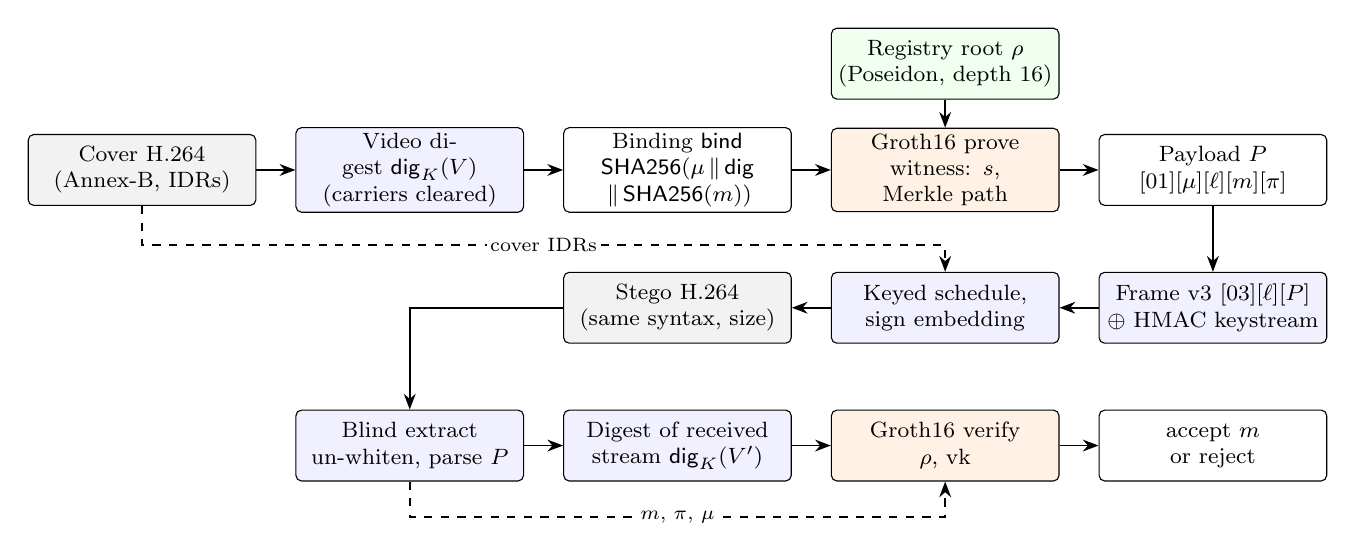
\begin{tikzpicture}[
  box/.style={draw, rounded corners=2pt, align=center, font=\footnotesize, minimum height=9mm,
              text width=2.75cm, inner sep=2pt},
  sec/.style={box, fill=blue!6},
  zk/.style={box, fill=orange!10},
  io/.style={box, fill=gray!10},
  arr/.style={-{Stealth[length=2mm]}, semithick},
  lab/.style={font=\scriptsize, fill=white, inner sep=1pt}]
% sender (top row, left to right)
\node[io]  (cover) at (0,0)    {Cover H.264\\(Annex-B, IDRs)};
\node[sec] (dig)   at (3.4,0)  {Video digest $\dig_K(V)$\\(carriers cleared)};
\node[box] (bind)  at (6.8,0)  {Binding $\bind$\\$\Hash(\mu\cat\dig$\\$\cat\Hash(m))$};
\node[zk]  (prove) at (10.2,0) {Groth16 prove\\witness: $s$, Merkle path};
\node[box] (pack)  at (13.6,0) {Payload $P$\\$[01][\mu][\ell][m][\pi]$};
\node[box, fill=green!6] (reg) at (10.2,1.35) {Registry root $\rho$\\(Poseidon, depth 16)};
% channel (middle row, right to left)
\node[sec] (frame) at (13.6,-1.75) {Frame v3 $[03][\ell][P]$\\$\oplus$ HMAC keystream};
\node[sec] (embed) at (10.2,-1.75) {Keyed schedule,\\sign embedding};
\node[io]  (stego) at (6.8,-1.75)  {Stego H.264\\(same syntax, size)};
% receiver (bottom row, left to right)
\node[sec] (extract) at (3.4,-3.5)  {Blind extract\\un-whiten, parse $P$};
\node[sec] (vdig)    at (6.8,-3.5)  {Digest of received\\stream $\dig_K(V')$};
\node[zk]  (verify)  at (10.2,-3.5) {Groth16 verify\\$\rho$, vk};
\node[box] (out)     at (13.6,-3.5) {accept $m$\\or reject};
\draw[arr] (cover) -- (dig); \draw[arr] (dig) -- (bind); \draw[arr] (bind) -- (prove);
\draw[arr] (prove) -- (pack); \draw[arr] (reg) -- (prove);
\draw[arr] (pack) -- (frame); \draw[arr] (frame) -- (embed); \draw[arr] (embed) -- (stego);
\draw[arr, dashed] (cover.south) -- ++(0,-0.5) -| node[lab, pos=0.25] {cover IDRs} (embed.north);
\draw[arr] (stego.west) -| (extract.north);
\draw[arr] (extract) -- (vdig); \draw[arr] (vdig) -- (verify); \draw[arr] (verify) -- (out);
\draw[arr, dashed] (extract.south) -- ++(0,-0.45) -| node[lab, pos=0.25] {$m$, $\pi$, $\mu$} (verify.south);
\end{tikzpicture}
\caption{Data flow. Blue: covert channel under the stego key $K$; orange: zero-knowledge proof; the verifier never sees $s$.}
\label{fig:overview}
\end{figure*}

\subsection{Keys}
From the 32-byte stego key $K$ the channel derives two subkeys with HKDF-SHA256~\cite{rfc5869}:
\begin{align}
\mathit{PRK}&=\HMAC(\texttt{"zkstego-cavlc-v2-salt"},K),\\
k_{\mathrm{sch}}&=\mathsf{Expand}(\mathit{PRK},\texttt{".../schedule"},32),\\
k_{\mathrm{wh}}&=\mathsf{Expand}(\mathit{PRK},\texttt{".../whitening"},32).
\end{align}
The camera secret $s$ is an independent uniformly random non-zero element of the BN254 scalar field; its public key is $pk=\Pos(s)$.

\subsection{Candidates and segments}
Each IDR picture together with its preceding SPS and PPS forms a \emph{segment}. A native parser decodes the CAVLC syntax of the IDR slice and lists one candidate per $4\times4$ (or $2\times2$ chroma DC) block that has a trailing one: the RBSP offset of its first \texttt{trailing\_ones\_sign\_flag}. A candidate is identified by the string $\mathit{id}=\texttt{nal:mb:category:block:bit}$ of its analysis NAL index, MB address, category (LumaDC, Luma4$\times$4/AC, ChromaDC, ChromaAC), block index and RBSP bit offset. By Proposition~\ref{prop:syntax} the identifiers are the same before and after embedding.

\subsection{Keyed schedule}
Within segment $j$ with candidate set $\mathcal C_j$, every candidate gets the score $\sigma(\mathit{id})=\HMAC(k_{\mathrm{sch}},\mathit{id})$; candidates are sorted by $(\sigma,\mathit{id})$ and the first $n_j=\min(\mathit{cap},|\mathcal C_j|)$ are selected. Frame bits are assigned to segments in order: segment $j$ carries frame bits $[\sum_{i<j}n_i,\ \sum_{i\le j}n_i)$ until the frame ends. The schedule depends only on $K$, the stream syntax and the per-IDR cap (64 bits by default), so a receiver reconstructs it from the stego stream alone, and the same procedure runs on a live stream as each IDR arrives.

\subsection{Frame and whitening}
The channel frame (protocol version 3) is
\begin{equation}
F=\texttt{0x03}\cat \mathrm{u16}(|P|)\cat P,
\end{equation}
with no MAC. Bit $i$ of $F$ (MSB first, counted across segments) is XORed with bit $i$ of the keystream $\HMAC(k_{\mathrm{wh}},\mathrm{u64}(0))\cat\HMAC(k_{\mathrm{wh}},\mathrm{u64}(1))\cat\cdots$ and written as the sign of the $i$-th scheduled candidate. Whitening makes the embedded bits pseudo-random, so about half of the scheduled signs actually change, and a wrong key yields a random version byte and length, which the extractor rejects. Authentication of the payload is left entirely to the proof; an earlier version carried a 16-byte HMAC tag, which cost 128 bits (two IDRs at the default cap) and added nothing once the proof binds the message.

\subsection{Camera registry}
The registry is a binary Merkle tree of depth 16 whose leaves are camera public keys (unused leaves are 0) and whose internal nodes are $\Pos(\ell,r)$. Verifiers trust only the root $\rho$; a camera's membership witness is its sibling path $(\mathit{sib}_t,\beta_t)_{t<16}$.

\subsection{Carrier-masked video digest}
Let $\Gamma_K(V)$ be the set of (NAL, RBSP bit) positions that the schedule of $K$ selects to carry the $L_F=8|F|$ frame bits of a payload of the given length. With the domain string $\mathsf{dom}_v=\texttt{"zkstego/video-digest/v1"}$, the digest is
\begin{align}
\dig_K(V)=\Hash\big(&\mathsf{dom}_v\cat\mathrm{u32}(L_F)\cat\mathrm{u32}(\mathit{cap})\nonumber\\
&\cat\textstyle\big\|_{u\in V}\,\mathrm{u32}(1+|r'_u|)\cat h_u\cat r'_u\big),
\label{eq:digest}
\end{align}
where for each NAL unit $u$ in file order $h_u$ is its header byte and $r'_u$ its RBSP with every bit in $\Gamma_K(V)$ cleared. The schedule depends on the syntax only, so $\Gamma_K(V)=\Gamma_K(V^{\star})$ for a cover $V$ and its stego $V^{\star}$.

\subsection{Binding, statement and payload}
For a mode $\mu\in\{0,1\}$ (0: video-bound; 1: message-only, Section~\ref{sec:discussion}) the binding, with $\mathsf{dom}_b=\texttt{"zkstego/proof-binding/v1"}$, is
\begin{equation}
\bind=\Hash(\mathsf{dom}_b\cat\mu\cat \dig_K(V)\cat\Hash(m)),
\end{equation}
split into two 128-bit field elements $(\bind_{\mathrm{hi}},\bind_{\mathrm{lo}})$. The circuit proves
\begin{multline}
\mathcal R=\{(\rho,\bind_{\mathrm{hi}},\bind_{\mathrm{lo}};\ s,\mathit{sib},\beta):\\
\mathsf{MerkleRoot}(\Pos(s),\mathit{sib},\beta)=\rho\ \wedge\ \beta_t\in\{0,1\}\}.
\end{multline}
The binding halves are public inputs that enter the R1CS through a squaring constraint, so a proof verifies only for the binding it was produced for. The circuit has 8{,}737 constraints and three public inputs. The payload is
\begin{equation}
P=\texttt{0x01}\cat\mu\cat\mathrm{u16}(|m|)\cat m\cat\pi,\qquad|\pi|=129,
\end{equation}
so $L_F=8(|m|+136)$; a 68-byte message gives $|P|=201$, $|F|=204$ bytes, 1{,}632 bits, i.e.\ 26 IDRs at 64 bits each.

\subsection{Channel parameters: selection policy and key mode}
\label{sec:params}
Two optional parameters are agreed out of band, like the cap; their defaults reproduce the channel described so far byte for byte.

\textbf{Selection policy.} Policy \texttt{random} ranks a segment's candidates by $(\sigma,\mathit{id})$. Policy \texttt{low-drift} ranks them by $(\tau,\sigma,\mathit{id})$, where the integer \emph{drift tier}
\begin{equation}
\tau=r+d+f\in\{0,\dots,5\}
\label{eq:tier}
\end{equation}
is derived from the distortion model of Section~\ref{sec:distortion}: $r=2,1,0$ for an MB row in the top, middle or bottom third of the picture (more blocks predict from upper rows), $d=2$ for the DC paths LumaDC and ChromaDC (their change covers a whole MB component), and $f=1$ when the flipped AC coefficient has $i+j\le2$ (low frequencies change the right column and bottom row used for prediction). All three inputs are syntax that sign flips never change, so the receiver recomputes the tiers from the stego stream; inside a tier the order stays keyed.

\textbf{Per-video keys and verification tokens.} In key mode \texttt{per-video} the subkeys are bound to the video. With $\nu=\Hash(\texttt{"zkstego/video-nonce/v1"}\cat\ldots)$ computed like Eq.~\eqref{eq:digest} over the SPS, PPS and first IDR of the stream with \emph{all} trailing-one sign candidates cleared (so $\nu$ is the same for cover and stego and independent of any key),
\begin{align}
\mathit{PRK}'&=\mathsf{Extract}(\texttt{"...-v4-salt"},K),\nonumber\\
k_v&=\mathsf{Expand}(\mathit{PRK}',\ \texttt{".../video"}\cat\nu,32),\nonumber\\
k_{\mathrm{sch}}&=\mathsf{Expand}(k_v,\texttt{".../schedule"},32),\nonumber\\
k_{\mathrm{wh}}&=\mathsf{Expand}(k_v,\texttt{".../whitening"},32).
\end{align}
The pair $t_V=(k_{\mathrm{sch}},k_{\mathrm{wh}})$ is the \emph{verification token} of video $V$. Anyone given $t_V$ can extract the payload of $V$ and compute $\dig$ of $V$ (Algorithm~\ref{alg:verify} with $t_V$ in place of $K$) and so verify its proof publicly, without learning $K$ or the token of any other video. A live stream obtains $\nu$ from its first segment as it arrives. The verify job accepts a token in place of the key in this mode.

\subsection{Algorithms}

\begin{algorithm}[t]
\caption{Embed (sender)}\label{alg:embed}
\begin{algorithmic}[1]
\Require cover $V$, message $m$, stego key $K$, camera $(s,\mathit{path})$, cap
\State $L_F\gets 8(|m|+136)$;\ $\Gamma\gets$ schedule$(V,K,L_F,\mathit{cap})$
\State $\delta\gets\dig_K(V)$ \Comment{Eq.~\eqref{eq:digest}}
\State $\bind\gets\Hash(\text{dom}\cat 0\cat\delta\cat\Hash(m))$
\State $\pi\gets\mathsf{Groth16.Prove}(\rho,\bind;\ s,\mathit{path})$
\State $F\gets\texttt{03}\cat\mathrm{u16}(|P|)\cat P$ with $P=\texttt{01}\cat0\cat\mathrm{u16}(|m|)\cat m\cat\pi$
\For{$i=0$ \textbf{to} $L_F-1$}
  \State set the sign at $\Gamma[i]$ to $F_i\oplus \mathit{ks}_i$
\EndFor
\State \Return $V^{\star}$
\end{algorithmic}
\end{algorithm}

\begin{algorithm}[t]
\caption{Verify (receiver)}\label{alg:verify}
\begin{algorithmic}[1]
\Require stream $V'$, $K$, root $\rho$, verification key vk, cap
\State read the first 24 scheduled bits, un-whiten; \textbf{reject} unless version $=3$ and length is admissible
\State read and un-whiten the remaining bits; parse $P$; \textbf{reject} if malformed
\If{$\mu=1$ and message-only proofs are not allowed} \textbf{reject}\EndIf
\State $\delta'\gets\dig_K(V')$ with $L_F$ from the header
\State $\bind'\gets\Hash(\text{dom}\cat\mu\cat\delta'\cat\Hash(m))$
\State \Return $\mathsf{Groth16.Verify}(\mathrm{vk},(\rho,\bind'_{\mathrm{hi}},\bind'_{\mathrm{lo}}),\pi)$
\end{algorithmic}
\end{algorithm}

Algorithms~\ref{alg:embed} and~\ref{alg:verify} summarize sender and receiver. The service exposes the verifier as an asynchronous job whose outcomes are \texttt{payload\_not\_found}, \texttt{malformed\_proof\_payload}, \texttt{video\_binding\_required}, \texttt{video\_digest\_unavailable}, \texttt{proof\_invalid} or acceptance with \texttt{video\_bound}; an extraction-only job returns the payload marked \texttt{verified: false}.

\section{Security Analysis}
\label{sec:security}

We argue goals G1--G5 informally under standard assumptions: SHA-256 and the Poseidon Merkle tree are collision resistant, Poseidon is one-way on uniformly random inputs, HMAC-SHA256 is a PRF, and Groth16 is perfectly zero-knowledge and weakly simulation-extractable: an adversary that has seen proofs for some public inputs can re-randomize them, but cannot produce an accepting proof for a \emph{new} public input without knowing a witness~\cite{baghery2021groth16}.

\begin{proposition}[Validity, G1]
\label{prop:validity}
Embedding changes only bits in $\Gamma_K(V)$; the stego stream parses into the same syntax elements with the same lengths as the cover, and only the selected trailing-one levels change sign.
\end{proposition}
\begin{proof}
Every bit in $\Gamma_K(V)$ is a \texttt{trailing\_ones\_sign\_flag}; apply Proposition~\ref{prop:syntax} once per flip, in any order.
\end{proof}

\begin{lemma}[Digest invariance]
\label{lem:invariance}
For a cover $V$ and its stego stream $V^{\star}$ under key $K$, $\dig_K(V^{\star})=\dig_K(V)$.
\end{lemma}
\begin{proof}
By Proposition~\ref{prop:validity} both streams have the same NAL units, headers and RBSP lengths (emulation-prevention bytes are not part of the RBSP), and the same candidates, so the schedule yields $\Gamma_K(V^{\star})=\Gamma_K(V)$. Their RBSPs differ only inside this set, which Eq.~\eqref{eq:digest} clears in both.
\end{proof}

\begin{lemma}[Syntax determines the mask]
\label{lem:mask}
If $\dig_K(V')=\dig_K(V)$ for a stream $V'$, then, except with negligible probability, $V'$ and $V$ have the same NAL units and RBSP lengths and differ only at positions in $\Gamma_K(V)=\Gamma_K(V')$.
\end{lemma}
\begin{proof}
Collision resistance of SHA-256 gives equal canonical strings, hence equal headers and lengths, and RBSPs that agree outside $\Gamma_K(V)\cup\Gamma_K(V')$. Consider the first differing bit in parsing order. Both streams parse identically up to it, so it has the same syntactic role in both; it lies in one of the two masks, hence it is a trailing-one sign flag in both. By Proposition~\ref{prop:syntax} the parse of the rest is unaffected, and induction over the differing bits shows that $V$ and $V'$ have identical syntax and candidates. The schedule depends only on syntax and $K$, so the masks are equal.
\end{proof}

\begin{theorem}[Binding, G2]
\label{thm:binding}
Suppose the verifier accepts $(V',m')$ in mode 0 and the adversary does not know the secret of any registered camera. Then, except with negligible probability, some registered camera produced a proof for a pair $(V,m)$ with $m'=m$ and $V'$ equal to $V$ (or to its honest stego stream) outside the carrier set $\Gamma_K(V)$.
\end{theorem}
\begin{proof}
Acceptance means a valid proof for $(\rho,\bind')$ with $\bind'=\Hash(\text{dom}\cat0\cat\dig_K(V')\cat\Hash(m'))$. If no honest proof was ever produced for $\bind'$, weak simulation-extractability yields a witness $(s',\mathit{path})$ whose leaf $\Pos(s')$ opens to $\rho$; by collision resistance of the tree the leaf is a registered key, and $s'$ is then a preimage of an honest camera's public key, contradicting one-wayness. Hence an honest camera proved $\bind'=\bind$ for some $(V,m)$. Collision resistance of SHA-256 gives $\Hash(m')=\Hash(m)$, so $m'=m$, and $\dig_K(V')=\dig_K(V)$; Lemma~\ref{lem:mask} concludes.
\end{proof}

\begin{remark}[What the carriers can still hold]
Theorem~\ref{thm:binding} leaves the carrier bits free, but those bits \emph{are} the payload: they must parse as a frame whose message is $m$ and whose proof verifies for $\bind$. An adversary can therefore at most replace $\pi$ by a re-randomized proof for the same statement. Flipping a carrier changes the extracted payload and is rejected (Section~\ref{sec:eval}); flipping any other bit changes the digest.
\end{remark}

\begin{corollary}[Attacks covered]
Each of the following yields rejection: embedding a valid payload into another video (the digest of the other video differs); dropping, appending or truncating NAL units; editing any non-carrier bit, including a trailing-one sign in a carrier IDR or any bit of a later frame; re-encoding; replacing the message; a proof made by a camera outside the trusted registry (it opens to a different root).
\end{corollary}

\begin{proposition}[Unforgeability with the stego key, G3]
Holding $K$ does not help produce an accepting proof for a new binding: $K$ enters only the schedule, the whitening and the mask, all of which are public to the verifier anyway, while acceptance requires a proof for $\bind$, which by the argument of Theorem~\ref{thm:binding} requires a registered secret.
\end{proposition}

This is the property a MAC-based design lacks: with a tag under $K$, every verifier can authenticate arbitrary content.

\begin{proposition}[Anonymity, G4]
The verifier's view---$\rho$, $\bind$ and $\pi$---has the same distribution for every registered camera.
\end{proposition}
\begin{proof}
$\rho$ and $\bind$ do not depend on which leaf is used. By perfect zero knowledge, $\pi$ can be simulated from the statement alone, so its distribution does not depend on the witness.
\end{proof}
Anonymity is relative to the registry: a registry of one camera identifies it.

\textbf{Covertness (G5).} Without $K$ the schedule is a pseudo-random subset of the candidates and the embedded bits are pseudo-random; with a wrong key the version byte matches with probability $2^{-8}$ and the length must additionally be admissible, after which the payload parser and the proof reject. Sign flips do not change the bit rate, the codeword lengths or the file size apart from rare emulation-prevention bytes. We only measure first-order statistics: the share of negative trailing ones does not change significantly (Section~\ref{sec:eval}). Calibrated or learned steganalysis is future work, and we do not claim security against it.

\textbf{Mode 1.} A live stream embeds its proof in the first IDRs, before the rest exists, so the proof can only bind the message. Theorem~\ref{thm:binding} then holds for $m$ but not for the video, and a mode-1 payload can be replayed into another stream. Verifiers reject mode 1 unless explicitly configured otherwise.

\section{A Distortion Model for Trailing-One Sign Embedding}
\label{sec:distortion}

The forward direction of the channel---choose candidates, embed, measure PSNR---does not tell a designer how many bits a frame can take before its quality drops below a target. This section derives the distortion of one flip in closed form, models its propagation, and inverts the result into a per-IDR bit budget. All energies are sums of squared errors (SSE) of 8-bit samples; $\PSNR=10\log_{10}(255^2 N_{\mathrm{px}}/\SSE)$ for a plane of $N_{\mathrm{px}}$ samples.

\subsection{Direct distortion of one flip}

\begin{lemma}[Single flip]
\label{lem:flip}
Flipping the sign of a trailing one at raster position $(i,j)$ of a $4\times4$ block coded with quantization parameter $\mathit{QP}$ changes the reconstructed residual of that block, before rounding and clipping, by an error of energy
\begin{equation}
E_{ij}=4\,\Qs(\mathit{QP})^2\,\kappa_m(i,j),
\label{eq:flip}
\end{equation}
\begin{equation}
\kappa_m(i,j)=\frac{v_m(i,j)^2\,\|b_i\|^2\|b_j\|^2}{16\,v_{m,0}^2},
\label{eq:kappa}
\end{equation}
with $m=\mathit{QP}\bmod6$. $\kappa_m(i,j)=1$ for the even/even class (including the DC position) and $\kappa_m(i,j)\in[0.925,1.057]$ for all positions and all $m$.
\end{lemma}
\begin{proof}
The level changes by $\Delta c=\mp2$. By Eq.~\eqref{eq:dequant} the scaled coefficient changes by $\Delta d=\mp2\,v_m(i,j)\,2^{\lfloor\mathit{QP}/6\rfloor}$ and no other coefficient changes. By linearity of Eq.~\eqref{eq:inverse} before the final rounding, the residual error is $\Delta e(x,y)=\Delta d\, b_i(x)\,b_j(y)/64$, whose energy is $(\Delta d/64)^2\|b_i\|^2\|b_j\|^2$. Substituting $\Qs=v_{m,0}2^{\lfloor\mathit{QP}/6\rfloor}/16$ gives Eq.~\eqref{eq:flip}. The bounds follow by evaluating the six tables: $\kappa\in\{1,1.056\}$, $\{1,1.012,1.046\}$, $\{0.925,0.947,1\}$, $\{1,1.033,1.054\}$, $\{0.954,0.977,1\}$ and $\{1,1.014,1.020\}$ for $m=0,\dots,5$.
\end{proof}

The near-constancy of $\kappa$ is not a coincidence: the scaling factors $v_m$ were designed to compensate the unequal norms of the integer basis~\cite{malvar2003transform}, so the scaled transform is close to orthonormal and, by Parseval, a level change of $\pm2$ costs $(2\Qs)^2$ wherever it occurs. The energy depends on the quantizer only; it does not depend on the image, the prediction mode or the frequency.

\begin{lemma}[DC paths]
\label{lem:dc}
A flip in an Intra16$\times$16 LumaDC block or a ChromaDC block has, before rounding, the same total energy $4\Qs^2$ (with $\mathit{QP}_c$ for chroma), spread uniformly over the sixteen (resp.\ four) $4\times4$ blocks of the MB component.
\end{lemma}
\begin{proof}
LumaDC: the Hadamard output changes by $\pm2$ in all sixteen positions, and the DC scaling $(f\cdot16v_{m,0}2^{\lfloor\mathit{QP}/6\rfloor})/64$ turns this into a change of $v_{m,0}2^{\lfloor\mathit{QP}/6\rfloor}/2$ in the DC coefficient of each block, i.e.\ a constant residual change of $v_{m,0}2^{\lfloor\mathit{QP}/6\rfloor}/128$ over each block; the total energy is $256\,(v_{m,0}2^{\lfloor\mathit{QP}/6\rfloor}/128)^2=4\Qs^2$. ChromaDC: the $2\times2$ Hadamard output changes by $\pm2$ in four positions, the scaling $(f\cdot16v_{m,0}2^{\lfloor\mathit{QP}_c/6\rfloor})/32$ gives $v_{m,0}2^{\lfloor\mathit{QP}_c/6\rfloor}$ per block, and four blocks of sixteen samples give the same total.
\end{proof}

\textbf{Additivity.} The schedule uses one candidate per block, so two flips in the same block can only be a DC-path flip and an AC flip of the same MB component. Their errors are orthogonal (an AC basis function has zero mean, a DC change is constant over the block), so the direct energies add exactly. Rounding by $(\cdot+32)\gg6$ adds a bounded perturbation; in the demo block of Appendix~\ref{app:example} the exact rounded energy is 128 against a model value of 121.

\subsection{Propagation}
Ignoring clipping and the rounding of prediction, intra decoding is affine in the residual: in decoding order every block is its prediction (a linear function of earlier reconstructed samples) plus its residual. A direct error $\delta_k$ of flip $k$ therefore becomes a total error $\mu_k=(I-\mathcal P)^{-1}\delta_k$, where $\mathcal P$ is the strictly lower-triangular prediction operator of the frame, and deblocking adds a further, data-dependent smoothing. We define the \emph{propagation gain}
\begin{equation}
G_k=\frac{\|\mu_k\|^2}{4\Qs(\mathit{QP}_k)^2},
\end{equation}
which captures drift through intra prediction and deblocking ($G_k\approx\kappa_k$ when nothing propagates; rounding and clipping can push it slightly below). For a set of flips the total error is $\sum_k\mu_k$; cross terms $\langle\mu_k,\mu_l\rangle$ carry the signs of the flipped levels, which are those of the cover coefficients, and are zero-mean over the random keyed choice of carriers. Hence
\begin{equation}
\mathbb E[\SSE]\approx\sum_k 4\,\Qs(\mathit{QP}_k)^2\,G_k .
\end{equation}
$G_k$ depends on the prediction structure---MB type, prediction modes, block position, whether deblocking is on---which is why it is measured rather than derived (Section~\ref{sec:eval}).

\subsection{Forward model and inverse}
With constant QP, $N$ flips in the luma plane and a frame-level gain $\bar G$ (the geometric mean of $G_k$ fitted on data),
\begin{equation}
\PSNR_Y\approx10\log_{10}\frac{255^2\,W H}{4\,\bar G\,N\,\Qs(\mathit{QP})^2}.
\label{eq:forward}
\end{equation}
Three rules of thumb follow: doubling the number of flips costs $3.01$\,dB, raising QP by six costs $6.02$\,dB, and four times more pixels gain $6.02$\,dB at the same number of flips. Inverting Eq.~\eqref{eq:forward} for a target $T$:
\begin{equation}
N_{\max}(T)=\frac{255^2\,W H\,10^{-T/10}}{4\,\bar G\,\Qs(\mathit{QP})^2},\qquad
\mathit{cap}(T)=\frac{N_{\max}(T)}{p\,f_Y},
\label{eq:inverse-cap}
\end{equation}
where $p=1/2$ is the probability that a whitened bit changes the sign and $f_Y$ the share of luma candidates (a uniformly random schedule selects luma carriers at that rate). Chroma planes have their own budget with $\mathit{QP}_c$ and the chroma gain.

\textbf{Receiver computability.} A per-IDR cap is usable only if the receiver derives the same value from the stego stream. Eq.~\eqref{eq:inverse-cap} uses $W$, $H$, the slice QP, $f_Y$ and a protocol constant $\bar G$; by Proposition~\ref{prop:syntax} all of them are identical in the cover and the stego stream. An adaptive cap therefore needs no side information. The same constraint applies to any cost-aware schedule: costs may depend on positions, categories, MB types, prediction modes and coefficient magnitudes, but never on the sign values that carry data.

\subsection{Towards minimal-distortion embedding}
Eq.~\eqref{eq:flip} supplies an additive per-carrier cost $\rho_k=4\Qs(\mathit{QP}_k)^2\kappa_k\hat G_k$, with $\hat G_k$ predicted from invariant features (e.g.\ category and MB type). For a payload of $L$ bits, the distortion-limited sender of~\cite{filler2011stc,fridrich2007practical} changes carrier $k$ with probability $p_k=1/(1+e^{\lambda\rho_k})$, where $\lambda$ solves $\sum_k h(p_k)=L$ ($h$ the binary entropy) and the expected distortion is $\sum_kp_k\rho_k$; syndrome-trellis codes come close to this bound. Even without costs, matrix embedding reduces flips per bit: the present channel spends $1/2$ expected flip per bit, while a Hamming code with $r=3$ embeds three bits into seven carriers with $1-2^{-3}=0.875$ expected flips, i.e.\ $0.29$ flips per bit, a $10\log_{10}(0.5/0.29)\approx2.3$\,dB gain at equal payload. Candidates are plentiful (thousands per IDR against 64 used), so the larger carrier count is affordable. We leave syndrome coding to future work. A simple integer version of the cost, the drift tier of Eq.~\eqref{eq:tier}, is implemented as the \texttt{low-drift} selection policy (Section~\ref{sec:params}) and evaluated end to end in Section~\ref{sec:eval-compare}.

\section{Implementation}
\label{sec:impl}

\textbf{Native codec layer (C++17).} A self-contained H.264 Baseline parser splits Annex-B streams, removes emulation prevention, parses SPS, PPS and I-slices down to every CAVLC element, and lists candidates. The same library implements the segment protocol for files and for byte streams, the carrier-masked digest, and re-emission of patched NAL units with emulation prevention. Command-line tools read the 32-byte key from standard input, never from the command line: \texttt{embed-stream-auth-stdin}, \texttt{extract-stream-auth}, \texttt{video-digest}, live variants on stdin/stdout, and an inspection tool that prints NAL tables, per-block coefficients and per-segment candidates as JSON.

\textbf{Proof layer.} The circuit is written in Circom~2.1 with circomlib's Poseidon; proofs are generated and verified with snarkjs~0.7.6 on Node.js~22. The setup script uses the public Hermez Powers of Tau of size $2^{16}$~\cite{hermez_ptau}, pinned by its published BLAKE2b hash, followed by two Phase-2 contributions with fresh entropy, a final beacon and a \texttt{zkey verify}. Both contributions run on one machine, so this is a demonstration ceremony; a deployment needs independent contributors. The verifier and the registry code (Python) reproduce the native digest byte for byte; a Python reference of the schedule and whitening is checked against the native codec in the test suite.

\textbf{Service.} A FastAPI application exposes asynchronous HTTP jobs (embed, extract, verify) and a WebSocket endpoint that pipes an Annex-B byte stream through the live embedder. Keys and messages reach native processes only through standard input; job records store neither; artifacts are downloadable once. The verify job loads the registry root from configuration and accepts message-only proofs only when explicitly enabled.

\textbf{Channel parameters.} The selection policy and the key mode of Section~\ref{sec:params} are command-line flags of every embedding, extraction and digest command (defaults reproduce the earlier protocol byte for byte), a \texttt{video-token} command prints the verification token of a video, and the inspection tool reports each candidate's tier inputs so that the Python mirror can reproduce the native schedule exactly.

\textbf{Testing.} The test runner groups 161 checks into twelve phases (proof, native contract including Python--native equality of both policies and both key modes, CLI fixtures, VLC tables, service, HTTP/WebSocket, manifest security, scheduler, benchmark analysis including the distortion model, trust interfaces, demo arithmetic, demo smoke run), plus seven CTest cases for the native library (among them: per-video nonce identical for cover and stego, token extraction equal to master-key extraction, a token failing on another video). The evaluation code has its own tests, e.g.\ that each re-implemented baseline embeds exactly the message bits it claims. A terminal walkthrough performs 60 automated cross-checks, e.g.\ that FFmpeg's decoder and our parser agree on every MB type and QP, that a Python re-implementation of dequantization, inverse transform and intra prediction reproduces FFmpeg's samples, and that the Python and native digests agree.

\section{Evaluation}
\label{sec:eval}

\subsection{Setup}
All measurements ran on one laptop (Intel Core i7-12700H, 14 cores/20 threads, 25.4\,GB RAM, Windows~11) with FFmpeg~8.0.1 (x264 core~165), Node.js~22.20 and snarkjs~0.7.6. Sources are nine Xiph CIF sequences~\cite{xiph_media} (akiyo, city, coastguard, container, deadline, football, two foreman variants, hall\_monitor), 30 frames each, encoded at their native $352\times288$ and Lanczos-upscaled to $640\times480$ and $1280\times960$ (upscaled sequences test scaling, not native high-resolution content). The benchmark encoder is x264 \emph{ultrafast}/zerolatency, Constrained Baseline, QP~22 for P frames (the I-slice QP is 19), all-intra, one slice per IDR; this preset uses only Intra16$\times$16 MBs and no deblocking. Each case embeds a 68-byte message with its proof (payload 201\,B, 1{,}632 frame bits) at the default cap of 64 bits per IDR, i.e.\ into 26 of the 30 IDRs, under a fresh stego key and an 8-camera registry. Wall times include process start-up (Node.js for snarkjs).

\subsection{Functional results}
All 27 cases passed every acceptance check: native capacity scan, embedding, strict FFmpeg decoding (\texttt{-xerror}), blind extraction of the exact payload, a video-bound proof verified against the registry root with the digest recomputed from the stego file, rejection under a wrong key, and zero sign changes outside the keyed schedule (checked position by position). The stego file has exactly the size of the cover in all 27 cases. A separate end-to-end run on 300 CIF frames passed five of five trials.

\subsection{Embedding quality}
Table~\ref{tab:quality} reports PSNR-Y and SSIM~\cite{wang2004ssim} per frame, comparing the clean decode of the cover with the decode of the stego stream (incremental embedding distortion), and from the original source (encoding plus embedding). About half of the 1{,}632 scheduled signs change (808--823 on average), i.e.\ about 31 per carrying frame. No frame falls below the common 40\,dB reference. The encoder's own loss dominates: on average, cover$	o$stego PSNR is 12--15\,dB higher than source$	o$stego PSNR.

\begin{table}[t]
\centering
\caption{Per-frame quality over the 26 carrying frames of 9 sequences per resolution.}
\label{tab:quality}
\setlength{\tabcolsep}{4pt}
\begin{tabular}{@{}lccc@{}}
\toprule
& CIF & $640\times480$ & $1280\times960$ \\
\midrule
Cover$\to$stego PSNR-Y, min [dB] & 46.71 & 44.03 & 44.72 \\
Cover$\to$stego PSNR-Y, mean [dB] & 57.44 & 59.69 & 62.64 \\
Cover$\to$stego SSIM, min & 0.99871 & 0.99895 & 0.99960 \\
Source$\to$stego PSNR-Y, min [dB] & 41.48 & 41.62 & 42.94 \\
Source$\to$stego PSNR-Y, mean [dB] & 45.57 & 46.43 & 48.11 \\
Changed signs per case (mean) & 808 & 823 & 816 \\
Candidates per case (mean) & 149{,}374 & 420{,}193 & 1{,}287{,}323 \\
\bottomrule
\end{tabular}
\end{table}

\subsection{Validating the distortion model}
\label{sec:eval-distortion}

We test the model of Section~\ref{sec:distortion} in three experiments (scripts and raw data in the artifact): (B)~single flips decoded in isolation, which measure the direct energy and the gain of individual carriers; (A)~the 27 benchmark encodes, which measure frame-level distortion with $\sim$22 luma flips per frame; and (C)~an inverse check that sets the cap from a target PSNR, embeds and measures.

\textbf{Experiment B: single flips.} We encoded the first frame of \emph{foreman} and \emph{city} (CIF) with two x264 configurations---\emph{ultrafast} (Intra16$\times$16 only, deblocking off; the benchmark encoder) and \emph{medium} (Intra4$\times$4 and Intra16$\times$16, deblocking on)---at QP~22, 28 and 34 (I-slice QP 19, 25, 31), sampled 100 candidates per encode (1{,}200 in total, skipping the rare carriers whose flip would add or remove an emulation-prevention byte), flipped each one alone and decoded with and without the loop filter.

\emph{Direct energy.} For all 385 sampled Intra4$\times$4 luma carriers, the change of the flipped block's own samples in the unfiltered decode equals, sample for sample, the change of the residual computed from Eqs.~\eqref{eq:dequant} and~\eqref{eq:inverse} with rounding; the decoder adds nothing else to the block. The ratio of that exact energy to the model value $4\Qs^2$ has median $1.012$ and mean $1.022$ (5th--95th percentile 0.95--1.19; small residuals are the most affected by rounding), and the pre-rounding factor $\kappa$ of the sampled positions lies in $[1.000,1.056]$, as Lemma~\ref{lem:flip} states.

\emph{Gains.} Table~\ref{tab:single} summarizes $G$. Three observations matter for the model. First, $G$ does not depend on QP (luma mean 6.6, 7.4, 6.0 for ultrafast and 38.4, 33.3, 34.0 for medium at the three QPs), so distortion scales as $\Qs^2$, i.e.\ by 6\,dB per six QP steps. Second, the gain is heavy-tailed: the median carrier barely propagates ($G\approx1$--$2$), but single luma gains reach 309 (ultrafast) and 2{,}187 (medium), and the 10\% largest gains account for 80\% (ultrafast) and 84\% (medium) of the total energy. Third, the encoder configuration matters more than anything else: the mean luma gain is 6.6 with Intra16$\times$16 only and 35.2 with Intra4$\times$4, whose nine directional modes chain many blocks. Deblocking changes the mean luma gain by about 1\% (35.6 without, 35.2 with), so drift through intra prediction, not filtering, is the propagation mechanism.

\begin{table}[t]
\centering
\caption{Single-flip propagation gain $G$ by carrier category (experiment B; $n$ flips, mean, median, 90th percentile).}
\label{tab:single}
\setlength{\tabcolsep}{4pt}
\begin{tabular}{@{}lrrrr@{\quad}rrrr@{}}
\toprule
& \multicolumn{4}{c}{ultrafast} & \multicolumn{4}{c}{medium} \\
Category & $n$ & mean & med. & p90 & $n$ & mean & med. & p90 \\
\midrule
Luma AC / 4$\times$4 & 352 & 3.7 & 1.04 & 5.7 & 395 & 35.4 & 2.1 & 52.9 \\
LumaDC & 38 & 33.8 & 4.9 & 64.4 & 5 & 16.3 & 12.6 & 31.6 \\
ChromaAC & 173 & 9.2 & 1.12 & 11.9 & 146 & 4.4 & 1.06 & 5.4 \\
ChromaDC & 37 & 23.9 & 7.1 & 65.3 & 54 & 30.5 & 11.4 & 102.2 \\
\midrule
All luma & 390 & 6.6 & 1.05 & 7.8 & 400 & 35.2 & 2.2 & 47.5 \\
\bottomrule
\end{tabular}
\end{table}

\begin{figure}[t]
\centering
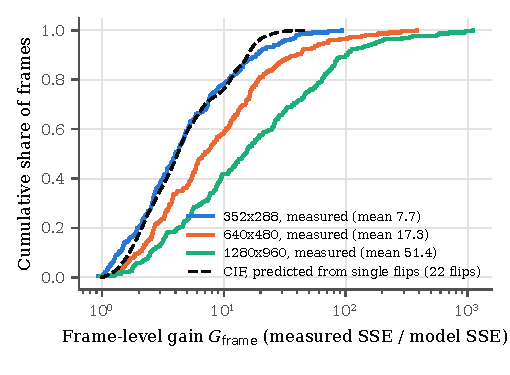
\includegraphics[width=\linewidth]{figures/frame_gain_cdf.pdf}
\caption{Frame-level gain of the 702 benchmark frames with luma flips (experiment A), and its prediction for CIF from single flips alone (experiment B, 22 independent draws per frame).}
\label{fig:framegain}
\end{figure}

\begin{figure*}[t]
\centering
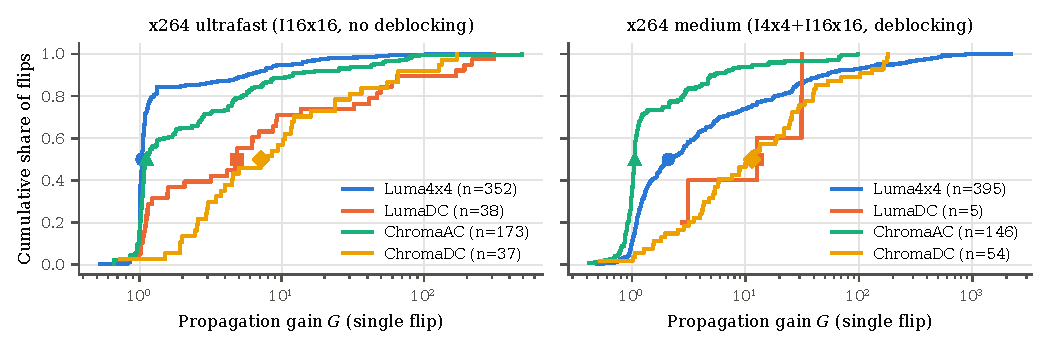
\includegraphics[width=\textwidth]{figures/gain_cdf.pdf}
\caption{Distribution of single-flip gains per carrier category for the two encoder configurations (markers: medians).}
\label{fig:gaincdf}
\end{figure*}

\textbf{Experiment A: sequences.} For each of the 810 frames of the benchmark we located every changed bit in the bitstream, classified it with the parser, summed the model energy $4\Qs^2$ per plane and compared it with the measured SSE between the cover and stego decodes. Table~\ref{tab:sequence} reports the frame-level gain. Its \emph{mean} (the ratio of total measured to total predicted energy) is the quantity Eq.~\eqref{eq:forward} needs; for CIF it is 7.7, close to the single-flip mean of 6.6 measured on different frames in experiment B. More strikingly, Fig.~\ref{fig:framegain} shows that drawing 22 single-flip gains at random reproduces the whole distribution of the CIF frame gains up to its 90th percentile (median 4.17 predicted vs.\ 4.00 measured); the measured upper tail is heavier (95th percentile 28.6 vs.\ 18.4), because carriers of the same frame share its content and are not independent. The gain grows with resolution (7.7, 17.3, 51.4). Our upscaled sequences contain large smooth regions, where Intra16$\times$16 prediction carries a change across many MBs; native high-resolution content may behave differently, and calibrating $\bar G$ per resolution and encoder is necessary.

Because a frame's distortion is dominated by its few high-gain carriers, the model predicts the \emph{distribution} of frame PSNR, not individual frames: with the per-resolution mean gain, the per-frame PSNR error has a mean absolute value of 4.1--6.7\,dB and a correlation of only 0.19--0.35 with the measurement (leave-one-sequence-out errors are the same to 0.05\,dB, so the gain does not overfit a sequence).

\begin{table}[t]
\centering
\caption{Frame-level gain in the 27-encode benchmark (experiment A, ultrafast, 64 bits per IDR).}
\label{tab:sequence}
\setlength{\tabcolsep}{4pt}
\begin{tabular}{@{}lccc@{}}
\toprule
& CIF & $640\times480$ & $1280\times960$ \\
\midrule
Frames with luma flips & 234 & 234 & 234 \\
Luma flips per frame & 22.0 & 22.7 & 22.9 \\
Mean gain $\bar G$ & 7.7 & 17.3 & 51.4 \\
Frame gain, median & 4.0 & 7.0 & 15.2 \\
Frame gain, 95th pct. & 28.6 & 65.8 & 173.8 \\
Measured PSNR-Y, median [dB] & 57.9 & 60.1 & 62.7 \\
Per-frame error, MAE [dB] & 4.1 & 5.1 & 6.7 \\
\bottomrule
\end{tabular}
\end{table}

\textbf{Experiment C: the inverse.} We encoded 30 frames of \emph{foreman} (CIF) with both configurations, computed the cap with Eq.~\eqref{eq:inverse-cap} for $T=40$, 45 and 50\,dB under three choices of the gain, embedded a random payload filling the capacity, and repeated each setting with five independent keys and payloads (145 fully loaded frames per setting): (i)~\emph{expected}, the mean single-flip gain of experiment B, which makes the expected frame energy equal to the budget; (ii)~\emph{p95-MC}, the 95th percentile of the frame gain obtained by Monte Carlo from single flips; (iii)~\emph{p95-sequence} (ultrafast only), the 95th percentile of the measured CIF frame gains of experiment A. The single-flip gains are pooled over both sources and all three QPs, which Table~\ref{tab:single} justifies for QP (the QP-19 subset has mean luma gain 6.6 and 38.4 against 6.6 and 35.2 pooled); the pool contains the first frame of \emph{foreman} but none of the other 29 test frames. The third policy uses data that include these frames' sequence. A cap at or above the number of candidates in an IDR (about 650 for ultrafast and 460 for medium here) saturates: every candidate is used and the target no longer controls anything.

\begin{table}[t]
\centering
\caption{Inverse check (experiment C): gain used, cap, share of frames with PSNR-Y $\ge T$ and 5th-percentile PSNR-Y [dB]; $^{s}$: cap at or above the candidate count of at least 97\% of the frames' IDRs (saturated).}
\label{tab:inverse}
\footnotesize\setlength{\tabcolsep}{3.2pt}
\begin{tabular}{@{}llrrrrr@{}}
\toprule
Encoder & Policy & $G$ & $T$ & cap & $\ge T$ & p05 \\
\midrule
\multirow{6}{*}{medium} & expected & 35.2 & 45 & 200 & 61\% & 40.2 \\
& expected & 35.2 & 50 & 63 & 70\% & 45.1 \\
& p95-MC & 63.4 & 40 & 351 & 86\% & 38.3 \\
& p95-MC & 102.4 & 45 & 68 & 88\% & 43.2 \\
& p95-MC & 140.1 & 50 & 15 & 86\% & 43.6 \\
& expected & 35.2 & 40 & 634$^{s}$ & 75\% & 37.3 \\
\midrule
\multirow{5}{*}{ultrafast} & expected & 6.6 & 50 & 311 & 46\% & 44.3 \\
& p95-MC & 15.8 & 50 & 130 & 80\% & 47.4 \\
& p95-seq. & 28.6 & 45 & 228 & 92\% & 43.7 \\
& p95-seq. & 28.6 & 50 & 72 & 91\% & 48.8 \\
& all three & -- & 40 & $\ge$721$^{s}$ & 99\% & 41.5 \\
\bottomrule
\end{tabular}
\end{table}

\begin{figure*}[t]
\centering
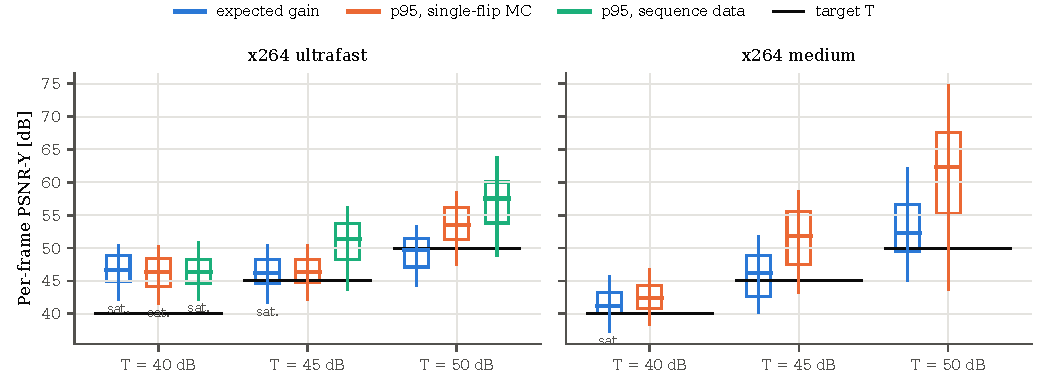
\includegraphics[width=0.8\textwidth]{figures/inverse_check.pdf}
\caption{Per-frame PSNR-Y for caps derived from a target $T$ (boxes: quartiles; whiskers: 5th--95th percentiles; 145 frames per box).}
\label{fig:inverse}
\end{figure*}

Table~\ref{tab:inverse} and Fig.~\ref{fig:inverse} give the outcome. The \emph{expected} policy places the median frame near the target, as intended (46--70\% of frames reach $T$). A percentile policy trades capacity for reliability: with the Monte Carlo percentile 80--88\% of frames reach $T$, short of the nominal 95\% for the reason seen in Fig.~\ref{fig:framegain} (correlated carriers within a frame), while the percentile measured on sequences reaches 91--92\%. Content is the other factor: the single-flip mean luma gain of \emph{foreman} alone at QP~19 is about twice the pooled value (12.9 vs.\ 6.6 for ultrafast, 70 vs.\ 35 for medium, $n\approx48$ each), so a gain calibrated on other content under-protects a sequence that propagates more. In every non-saturated setting the 5th percentile stays within 6.5\,dB below the target, and the cap moves in the direction and by the amount the model predicts: from $T=45$ to $50$\,dB the cap shrinks by $10^{0.5}\approx3.2\times$ under the expected policy (200 to 63, 983 to 311). Saturation itself is informative: at the benchmark's QP the ultrafast stream cannot drop below about 41.5\,dB at its 5th percentile even when every candidate is used.

\textbf{What the data suggest for carrier selection.} Since a tenth of the carriers produces four fifths of the distortion, excluding high-gain carriers is worth more than reducing the payload. The single-flip data show which invariant features predict the gain. In the medium configuration, low-frequency trailing ones (coefficient positions with $i+j\le1$) have mean gains of 84--92 against 1.6 at $i+j=6$, because low-frequency basis functions change the right column and bottom row from which later blocks predict. In both configurations, carriers in the top third of the picture have mean gains of 13.9 (ultrafast) and 65.6 (medium), against 2.2 and 6.1 in the bottom third, because more blocks are predicted from them. Restricting a random schedule to bottom-third carriers would reduce the expected energy by 4.8\,dB (ultrafast) and 7.6\,dB (medium) according to these averages, and excluding DC paths by 2.5\,dB (ultrafast). These are projections from single-flip averages, not end-to-end measurements; the cost-aware schedule they motivate keeps the receiver-computability constraint of Section~\ref{sec:distortion}.


\subsection{Sign statistics}
Over all candidate signs of a case, the share of negative trailing ones is $0.504$ before and after embedding; the two-proportion $z$-statistic is at most $0.223$ in absolute value over the 27 cases, far from the 1.96 threshold of a 5\% test. This is a first-order indicator only (Section~\ref{sec:discussion}).

\subsection{Performance}
Table~\ref{tab:zkp} compares Groth16 and PLONK on the same R1CS and witness; both verify a correct proof and reject a tampered public input. Groth16's 129-byte proof is what makes the covert channel practical: snarkjs serializes a PLONK proof as 2.25\,KB of JSON, which would need about 290 IDRs at the default cap, and even a compact binary encoding is several times larger than 129\,B. Table~\ref{tab:e2e} gives the end-to-end stages for 300 CIF frames. Native costs scale with the number of parsed IDRs: the median capacity scan takes 52, 220 and 770\,ms per IDR at the three resolutions, embedding 61, 245 and 891\,ms per carrying IDR, and the digest, which parses the 26 carrying IDRs, 1.6, 6.4 and 22.6\,s. Parsing, not proving, bounds throughput at high resolution; the parser is single-threaded and unoptimized.

\begin{table}[t]
\centering
\caption{Proof systems on the \texttt{camera\_video} circuit (8{,}737 constraints, 3 public inputs).}
\label{tab:zkp}
\begin{tabular}{@{}lcc@{}}
\toprule
& Groth16 & PLONK \\
\midrule
Trials & 5 & 3 \\
Prove [s] & 1.52--1.60 & 21.5--23.3 \\
Verify [s] & 0.91--1.01 & 0.90--0.94 \\
Proof size & 129\,B (compressed) & 2.25\,KB (JSON) \\
Peak prover RSS [MB] & 695 & 864 \\
Setup & circuit-specific (Phase 2) & universal SRS, 3.2\,s \\
Proving key & 4.2\,MB & 30.1\,MB \\
\bottomrule
\end{tabular}
\end{table}

\begin{table}[t]
\centering
\caption{End-to-end stages, 300 CIF frames, 5 trials (median, ms).}
\label{tab:e2e}
\begin{tabular}{@{}lr@{\qquad}lr@{}}
\toprule
\multicolumn{2}{@{}c}{Sender} & \multicolumn{2}{c@{}}{Receiver} \\
\midrule
Cover digest & 511 & Extract & 535 \\
Groth16 prove & 1{,}774 & Digest + verify & 1{,}448 \\
Embed & 500 & Strict decode & 150 \\
\textbf{Total} & \textbf{2{,}779} & \textbf{Total} & \textbf{1{,}989} \\
\bottomrule
\end{tabular}
\end{table}

\subsection{Attack matrix}
Table~\ref{tab:attacks} lists the attacks run through the service's verify job on the end-to-end stream. Only the untouched stream is accepted. Notably, flipping a sign that does not carry the frame---in an IDR that does carry it---is rejected through the digest, and so is the same valid payload embedded into another video; a camera that builds its own registry produces a proof that verifies against its own root but not against the trusted one.

\begin{table}[t]
\centering
\caption{Attack matrix (verify job outcome and reason).}
\label{tab:attacks}
\footnotesize
\begin{tabular}{@{}ll@{}}
\toprule
Case & Result (rejection reason) \\
\midrule
Untouched stego stream & accepted \\
Wrong stego key & \texttt{payload\_not\_found} \\
Flip a scheduled carrier sign & \texttt{malformed\_proof\_payload} \\
Flip non-carrier sign, carrier IDR & \texttt{proof\_invalid} \\
Flip a sign in a later frame & \texttt{proof\_invalid} \\
Drop the first IDR & \texttt{payload\_not\_found} \\
Truncate to half & \texttt{proof\_invalid} \\
Re-encode (transcode) & \texttt{payload\_not\_found} \\
Swap the message & \texttt{proof\_invalid} \\
Camera outside the registry & \texttt{proof\_invalid} \\
Replay into another video & \texttt{proof\_invalid} \\
\bottomrule
\end{tabular}
\end{table}

\section{Discussion and Limitations}
\label{sec:discussion}

\textbf{Where the design fits.} The scheme protects bitstreams that are moved without re-encoding: surveillance and body-camera evidence chains that archive the camera's H.264, files exchanged as files, and newsroom or legal workflows that need to show that footage comes from an authorized device without naming it. In these settings metadata is routinely lost while the elementary stream survives, and hiding the proof keeps an adversary from selectively removing it.

\textbf{Why not a SEI message?} A proof could be carried in a user-data SEI NAL unit at no capacity cost and with the same digest construction (the SEI unit would be excluded instead of the carrier bits). The difference is covertness: a SEI payload is visible to every parser and trivially stripped by a sanitizer, while the sign channel is located only with $K$. When covertness is not needed, the SEI variant is simpler, and our binding and proof carry over unchanged.

\textbf{Who can verify.} Extraction and the carrier mask depend on the stego key, so by default verification is limited to key holders, who still cannot forge proofs (G3). Per-video key mode (Section~\ref{sec:params}) makes verification of a chosen video public: its 64-byte token is handed to a court, a platform or published next to the file, and only that video loses its covertness. Fully keyless verification of every video would require the carrier set to be public, which contradicts hiding the payload.

\textbf{Fragility.} Any re-encode, resize or transcode destroys the payload and changes the digest. Robust provenance across edits requires transformation proofs~\cite{photoproof2016,veritas2024,zkcinema2026} or a robust watermark acting as a soft binding~\cite{c2pa_spec}; combining such a layer with an in-band anonymous proof is an open direction.

\textbf{What the proof does not show.} A registered camera can film a screen; the camera secret lives in software in our prototype, so a compromised device can sign anything; registry governance (enrollment, revocation by publishing a new root, root distribution) is outside the system. Binding the secret to a secure element or an attested sensor pipeline, as in ZK-IMG~\cite{zkimg2022}, would address part of this.

\textbf{Live streams.} In mode 1 the proof binds the message only and can be replayed; video binding for live streams would need a proof that commits to frames embedded later, e.g.\ a chain of proofs or a final proof carried in a trailing segment.

\textbf{Codec scope.} The channel needs CAVLC and IDR frames. Most capture devices use the High profile with CABAC, where sign bits are bypass-coded but not length-invariant in the same simple way; HEVC uses sign data hiding, which interacts with sign embedding. Porting the channel is engineering work with its own distortion and syntax analysis.

\textbf{Trusted setup.} Groth16 needs a circuit-specific ceremony; our ceremony is a demonstration. PLONK removes the circuit-specific phase at a cost of roughly $14\times$ in proving time and a $2.25$\,KB proof (Section~\ref{sec:eval}), which no longer fits the covert channel at the default cap.

\textbf{Steganalysis.} Four detectors (compressed-domain features, SPAM, a reduced rich model, a CNN) are at chance at the default rate and succeed at 20\% of the candidates (Section~\ref{sec:eval-steg}). This bounds what moderately strong detectors trained on 17 sequences achieve, not what a determined warden with the full rich model, modern networks and large training sets could do~\cite{ker2013realworld}; covertness claims should stay tied to the default rate. Minimal-distortion coding with the costs of Section~\ref{sec:distortion} would reduce the number of changes and is the natural next defense.

\section{Conclusion}
\label{sec:conclusion}

We showed that a zero-knowledge proof of anonymous camera membership is small enough to be hidden in the trailing-one signs of an H.264 stream, and that it can be bound to the exact stream that carries it through a digest that masks only the keyed carrier positions. The resulting system needs no metadata, hides the signer within a registry, rejects replay, truncation, edits and re-encodes, and lets a verifier who holds the stego key check a proof that it cannot forge. We also derived a closed-form distortion model of sign embedding---one flip costs $4\Qs^2$ up to a factor in $[0.925,1.057]$---and turned it into a per-frame bit budget for a target PSNR, which our experiments confirm once the propagation gain of the encoder configuration is known. Future work includes minimal-distortion coding with the derived costs, steganalysis, CABAC and HEVC, hardware-bound camera secrets and video binding for live streams.

\section*{Artifact availability}
Source code, circuit, benchmark scripts and the recorded results used in this paper are available at \url{https://github.com/Saudadeeee/zk-snark-X-Steganography}.


\bibliographystyle{IEEEtran}
\bibliography{references}

\appendices
\section{Worked Example of One Carrier}
\label{app:example}

We follow one carrier of a demonstration run (\texttt{akiyo}, CIF, x264 default preset, I-slice QP 19, so $\Qs=5.5$ and $4\Qs^2=121$) from the bitstream to the pixels. The carrier is the first trailing-one sign of luma block~5 of MB~212 (Intra4$\times$4, prediction mode Diagonal\_Down\_Right), at RBSP bit 57{,}561 of the first IDR NAL unit.

\textbf{CAVLC.} With $n_C=6$ the block is coded as \texttt{coeff\_token}=\texttt{1011} (TotalCoeff 4, TrailingOnes 3), sign flags \texttt{0\,1\,1}, one level \texttt{1}, \texttt{total\_zeros}=\texttt{111} and two \texttt{run\_before} codes. The scheduled bit is the first sign flag; whitening requires a 1, so the flag becomes \texttt{1} and the flags read \texttt{1\,1\,1}. All other bits keep their position and meaning. In the file the byte at offset 7{,}805 changes from \texttt{bf} to \texttt{ff}.

\textbf{Levels and scaling.} The scan $(1,-1,0,-1,1,0,\dots)$ becomes $(1,-1,0,-1,-1,0,\dots)$: zig-zag position 4, raster $(1,1)$, an odd/odd coefficient. With $v_{1}(1,1)=18$ and $2^{\lfloor19/6\rfloor}=8$ the scaled coefficient changes from $144$ to $-144$:
\begin{equation*}
D=\begin{bmatrix}88&-112&0&0\\0&\pm144&0&0\\-88&0&0&0\\0&0&0&0\end{bmatrix}.
\end{equation*}

\textbf{Residual.} The inverse transform gives
\begin{equation*}
\hat e_{\mathrm{before}}=\begin{bmatrix}1&0&0&0\\2&2&3&3\\0&1&4&6\\-4&-2&2&4\end{bmatrix},\
\hat e_{\mathrm{after}}=\begin{bmatrix}-4&-2&2&4\\0&1&4&6\\2&2&3&3\\1&0&0&0\end{bmatrix},
\end{equation*}
a change of energy $\sum\Delta\hat e^2=128$. Lemma~\ref{lem:flip} predicts $4\Qs^2\kappa_1(1,1)=121\times1.046=126.6$ before rounding.

\textbf{Reconstruction.} A flip does not affect blocks decoded earlier, so if this were the only carrier the block's prediction would be unchanged and its samples would change by exactly $\Delta\hat e$ (Experiment~B confirms this for every sampled Intra4$\times$4 block). In the demo a block decoded earlier also carried a flip, which shows up as a uniform change of $+1$ in this block's prediction: an instance of intra drift. Our Python reconstruction (prediction plus residual) matches FFmpeg sample by sample before and after embedding, decoded with \texttt{-skip\_loop\_filter all}; deblocking then smooths the block edges.

\section{Notation}
\begin{table}[h]
\centering
\small
\begin{tabular}{@{}ll@{}}
\toprule
$K$, $s$ & stego key, camera secret \\
$k_{\mathrm{sch}}$, $k_{\mathrm{wh}}$ & schedule and whitening subkeys \\
$\rho$, $pk$ & registry root, camera public key $\Pos(s)$ \\
$\Gamma_K(V)$ & carrier positions of stream $V$ under $K$ \\
$\dig_K$, $\bind$ & carrier-masked digest, binding \\
$F$, $P$, $\pi$ & frame, payload, compressed proof \\
$\mathit{cap}$ & bits per IDR segment \\
$\Qs$, $v_m(i,j)$ & quantizer step, scaling factor \\
$\kappa$, $G$ & position factor, propagation gain \\
\bottomrule
\end{tabular}
\end{table}


\end{document}
